% ============================================================================
%  第 6 章  扩展 TFT
% ============================================================================
\chapter{扩展 TFT}\label{ch:06}

\begin{flushright}
\small 第 11 讲；2021 年 3 月
\end{flushright}

\begin{keytakeaways}
本章把前面反复出现的“分歧”现象从余维 1 提升到余维 2：闭 $(n-1)$-流形配一个向量空间，
而闭 $(n-2)$-流形配一个范畴。Atiyah--Segal 公理把一个对称幺半函子
$Z\colon(\Bord_{n-1,n},\sqcup)\to(\Vect,\otimes)$ 作为（非扩展）TFT 的定义，其配分函数沿余维 1
子流形粘合时的局部性，正好对应于 $Z(M_1\sqcup_N M_2)$ 的因子化；但要沿余维 2 的 $N$ 粘合状态空间，
就需要 2-层扩展场论 $Z\colon(\Bord_{n-2,n},\sqcup)\to(\cC,\otimes)$，并要求 $\cC$ 是 $\Vect$ 的
去环路（$\End_\cC(1_\cC)=\Vect$）。物理上，对 3-流形中的纽结 $K$ 取管状邻域边界 $N$，
边界上的层 $\cE_N$ 经拉回给出修改后的态空间 $\Gamma(M,\pi_N^*\cE_N)$；Dirichlet 与 von Neumann
边界条件分别对应摩天楼层与常值层。本章随后在两个阿贝尔对偶的二维例子与四维拓扑 Maxwell 理论中
验证这一机制，得到余维 2 的阿贝尔对偶即 Fourier--Mukai 变换
$\Loc(\operatorname{Pic}\Sigma)\simeq\QC(\Loc)$；最后把带分歧类域论表述为 $K_x^\times$ 的表示
与 $D_x^\times$ 上特征局部系统（层）之间的对应，为局部与整体类域论的几何化埋下伏笔。
\end{keytakeaways}

\section{分歧}

\begin{sectionkey}
本节回顾螺线管与 Dirac 单极子这两个物理上的分歧例子，并把“在边界上提条件”统一表述为
“在边界场空间上取一个层，再沿限制映射拉回并取整体截面”；余维 2 的数据由此第一次以范畴/层的面目出现。
\end{sectionkey}

我们已经在扩展 TFT 中见过分歧的概念，现在考虑更高余维的版本。这意味着我们正在
“提升范畴层次”，从向量空间提升到范畴。

这将把我们已经见过的某些例子形式化。在物理中我们有两个分歧的例子。
第一个是 Maxwell 理论中的\term{螺线管}{solenoid}概念。此时我们在流形 $M^3$ 中有某个纽结，
然后考虑 $H^2((M,N),\Z)$，其中 $N$ 是纽结的管状邻域的边界。其对偶为
\begin{equation}\tag{6.1}\label{eq:6.1}
H^2\bigl((M,N),\Z\bigr)^{\vee}\simeq H^1\bigl(M\setminus N,\C^{\times}\bigr).
\end{equation}
于是想法是：$H^2((M,N),\Z)$ 由配备纽结上平凡化的线丛组成，而
$H^1(M\setminus N,\C^{\times})$ 是沿纽结带奇点的平坦联络。

我们还有 Dirac 单极子，其中考虑 $H^2(M\setminus N,\Z)$，这里 $N$ 是一个小球的边界。
可以把它想成在该点带奇点的线丛。其对偶为
\begin{equation}\tag{6.2}\label{eq:6.2}
H^2\bigl(M\setminus N,\Z\bigr)^{\vee}\simeq H^1\bigl((M,N),\C^{\times}\bigr),
\end{equation}
我们可以把它理解为在该点带平凡化的平坦联络。

类似的事情出现在算术情形。我们有线丛与平坦联络之间的 Cartier 对偶：
\begin{equation}\tag{6.3}\label{eq:6.3}
\operatorname{Pic}(C)^{\vee}\simeq \Loc_1 C .
\end{equation}
在左边可以添加\term{水平结构}{level structure}，即在子集 $S\subset C$ 上添加平凡化。
在右边可以在 $S\subset C$ 处添加奇点。于是带分歧的类域论告诉我们：一边添加水平结构，
如何对应于另一边添加奇点。

现在我们想从物理观点更系统地解释如何添加高余维的数据。

回忆在场论中，我们研究流形 $M$ 上的场 $\cF(M)$。若 $M$ 有边界 $\partial M=N$，
则得到映射
\begin{equation}\tag{6.4}\label{eq:6.4}
\cF(M)\xrightarrow{\ \pi_N\ }\cF(N).
\end{equation}

% [Tutor Note: 这里及式 (6.5) 中 $\Gamma$ 的第一个变元其实是场空间 $\cF(M)$，而不是流形 $M$ 本身；
%  作者对 $M$ 与 $\cF(M)$ 的记号有混用。严格地说，(6.5) 应写作 $\Gamma(\cF(M),\pi_N^*\cE_N)$，
%  其中 $\pi_N\colon\cF(M)\to\cF(\partial M)$ 是限制映射。后文 (6.19)--(6.21) 改用 $\cF(\cdot)$ 才是准确写法。]

在（单极子和螺线管的）例子中，我们随后对 $N$ 提条件（要么允许奇点，要么要求平凡化）。
我们可以如下“一次性”地陈述。设 $\cE_N$ 是 $\cF(\partial M)$ 上任意层。回忆我们把一个向量空间
附着到 $M$，即 $\cF(M)$ 上函数（或上同调等）的向量空间。现在我们想用边界数据 $\cE_N$ 修改它。
具体地，我们可以把 $\cE_N$ 拉回到 $M$，得到 $\pi_N^*\cE_N$。这是 $M$ 上的层，
故可取整体截面得到新的向量空间
\begin{equation}\tag{6.5}\label{eq:6.5}
\Gamma\bigl(M,\pi_N^*\cE_N\bigr).
\end{equation}
这是附着到 $M$ 的 Hilbert 空间的修改版本。于是我们得到附着到 $M$ 与某个 $\cE_N$ 的数据的向量空间，
而 $\cE_N$ 扮演我们对 $N$ 所提条件（奇点或平凡化）的角色。

\begin{srcrem}{26}
对任意 $\pi\colon X\to Y$ 与 $\cE\in\Shv(Y)$，我们有
\begin{align}
\Gamma(X,\pi^*\cE)&=\Gamma(Y,\pi_*\pi^*\cE)\tag{6.6}\label{eq:6.6}\\
&=\Gamma(Y,\cE\otimes\pi_*k_X).\tag{6.7}\label{eq:6.7}
\end{align}
于是对任意 $X$ 都可附着 $\pi_*k_X\in\Shv(Y)$，与这个对象配对就给出一个向量空间；
或者我们也可以把这理解为通过拉回 $\cE$ 而附着到 $X$ 的向量空间。
\end{srcrem}

\subsection{拓扑 Maxwell 理论}

在拓扑 Maxwell 理论（第 4.8.1 节）中，A-侧处理的是
\begin{equation}\tag{6.8}\label{eq:6.8}
H^*\bigl(\cC(M)\bigr),
\end{equation}
其中 $\cC(M)$ 是 $M$ 上带联络的线丛构成的空间。现在修改它以还原相对版本，即
\begin{equation}\tag{6.9}\label{eq:6.9}
H^2\bigl((M,N),\Z\bigr)
\end{equation}
或
\begin{equation}\tag{6.10}\label{eq:6.10}
H^2\bigl(M\setminus N,\Z\bigr).
\end{equation}
回忆联络空间的分量由
\begin{equation}\tag{6.11}\label{eq:6.11}
\pi_0\cC(M)\simeq H^2(M,\Z)
\end{equation}
给出，故可以把 $H^2(M,\Z)$ 想成连通分量上的局部常值函数。要点是联络空间在拓扑上是
\begin{equation}\tag{6.12}\label{eq:6.12}
\cC(M)=\operatorname{Map}\bigl(M,K(\Z,2)\bigr)=\operatorname{Map}\bigl(M,BU(1)\bigr),
\end{equation}
故其分量由 $H^2(M,\Z)$ 给出。

于是 Maxwell 理论中的 Hilbert 空间是 $\cC(M)$ 上常值层的上同调。
现在想通过取不同层的上同调来修改它。我们有从 $M$ 到边界 $\partial M=N$ 的限制
\begin{equation}\tag{6.13}\label{eq:6.13}
\operatorname{Map}\bigl(M,K(\Z,2)\bigr)\xrightarrow{\ \pi_N\ }\operatorname{Map}\bigl(N,K(\Z,2)\bigr),
\end{equation}
故可以从边界上的层出发，把它拉回 $M$ 并取上同调。

例如，在
\begin{equation}\tag{6.14}\label{eq:6.14}
\operatorname{Map}\bigl(N,K(\Z,2)\bigr)=\operatorname{Map}\bigl(N,BU(1)\bigr)
\end{equation}
内部有常值映射，即存在一个点
\begin{equation}\tag{6.15}\label{eq:6.15}
i\colon \{\mathrm{pt}\}\hookrightarrow \operatorname{Map}\bigl(N,BU(1)\bigr),
\end{equation}
由把 $N$ 送到 $\mathrm{pt}\in BU(1)$ 的映射给出。考虑该点处的摩天楼层 $i_*\C$，并把它取作我们的层：
\begin{equation}\tag{6.16}\label{eq:6.16}
\cE_N=i_*\C .
\end{equation}
然后把它拉回 $M$ 得到 $\pi^*\cE_N$，其上同调为
\begin{equation}\tag{6.17}\label{eq:6.17}
H^*\bigl(\cC(M),\pi^*\cE\bigr)
=H^*\bigl(\text{$M$ 上的线丛，加上 $N$ 上的平凡化}\bigr).
\end{equation}
这是 Dirichlet 边界条件。特别地，我们可以把相对上同调 $H^2((M,N),\Z)$ 还原为如下纤维积的 $\pi_0$：
\begin{equation}\tag{6.18}\label{eq:6.18}
\begin{array}{ccc}
\square & \longrightarrow & \operatorname{Map}\bigl(M,K(\Z,2)\bigr)\\[2pt]
\downarrow & & \downarrow\\[2pt]
\mathrm{pt} & \longrightarrow & \operatorname{Maps}\bigl(M,K(\Z,2)\bigr)
\end{array}
\end{equation}

% [Tutor Note: 式 (6.18) 在原文中是不完整的：左上角只印出一个方框占位符，右下角写作
%  $\mathrm{Maps}(M,K(\Z,2))$。按上下文（相对上同调 = 纤维积的 $\pi_0$），左上应为纤维积
%  $X=\mathrm{pt}\times_{\operatorname{Map}(N,K(\Z,2))}\operatorname{Map}(M,K(\Z,2))$，
%  右下应为 $\operatorname{Map}(N,K(\Z,2))$（限制映射的靶）。这里照原文保留方框，
%  以便读者核对源文；理解时请按上述纤维积补全。]

设 $K\subset M$ 是一个纽结，$N$ 是 $K$ 的管状邻域的边界。记 $M_0$ 为去掉纽结后得到的、
以 $\partial M_0=N$ 为边界的流形。于是若要还原 $M_0$ 的上同调，只需取 $\cF(N)$ 上的常值层
并把它拉回到 $\cF(M_0)$。这是 von Neumann 边界条件。

重申一下：给定 $M$ 上的场，我们可以沿 $K\subset M$ 如下地加条件。我们有映射
\begin{equation}\tag{6.19}\label{eq:6.19}
\cF\bigl(M\setminus K=:M_0\bigr)\to\cF(\partial M_0),
\end{equation}
于是可以取右边的层，把它们拉回 $\cF(M_0)$，并取 $\cF(M_0)$ 以该层为系数的上同调。

例如，常值层 $\C$ 的拉回仍是常值层，然后我们取
\begin{equation}\tag{6.20}\label{eq:6.20}
H^*\bigl(\cF(M\setminus K),\pi^*\C=\C\bigr)=H^*\bigl(\cF(M\setminus K)\bigr),
\end{equation}
即我们允许沿 $K$ 有任意的奇点。

也可以考虑摩天楼层 $i_*\C$，其中 $i\colon \mathrm{pt}\hookrightarrow\partial M_0$。这给出
\begin{equation}\tag{6.21}\label{eq:6.21}
H^*\bigl(\cF(M\setminus K),\pi^*i_*\C\bigr)
=H^*\bigl(\text{联络，加上 $N$ 上的平凡化}\bigr).
\end{equation}

总之，我们可以把边界上的层看成给 $M$ 附着新向量空间的各种方式的来源。

\section{扩展 TFT}

\begin{sectionkey}
本节系统引入 Atiyah--Segal 公理与 2-层扩展场论：闭 $n$-流形给数、闭 $(n-1)$-流形给向量空间、
闭 $(n-2)$-流形给范畴；并说明 4 维 TFT 中的纽结如何通过“去掉管状邻域再沿边界加层”实现余维 2 的分歧。
\end{sectionkey}

$n$ 维 TFT 的粗略想法，是把一个数附着到闭 $n$-流形 $P$ 上。可以把它想成 $P$ 上所有场构成的
空间的某种体积。然后对闭 $(n-1)$-流形，我们附着了一个向量空间，并把它想成 $M$ 上场空间的泛函空间。
现在我们想对闭 $(n-2)$-流形附着某种范畴。这同样是场空间的某种线性化，
但现在是 $\cF(N)$ 上层的范畴。

\begin{figure}[htbp]
  \centering
  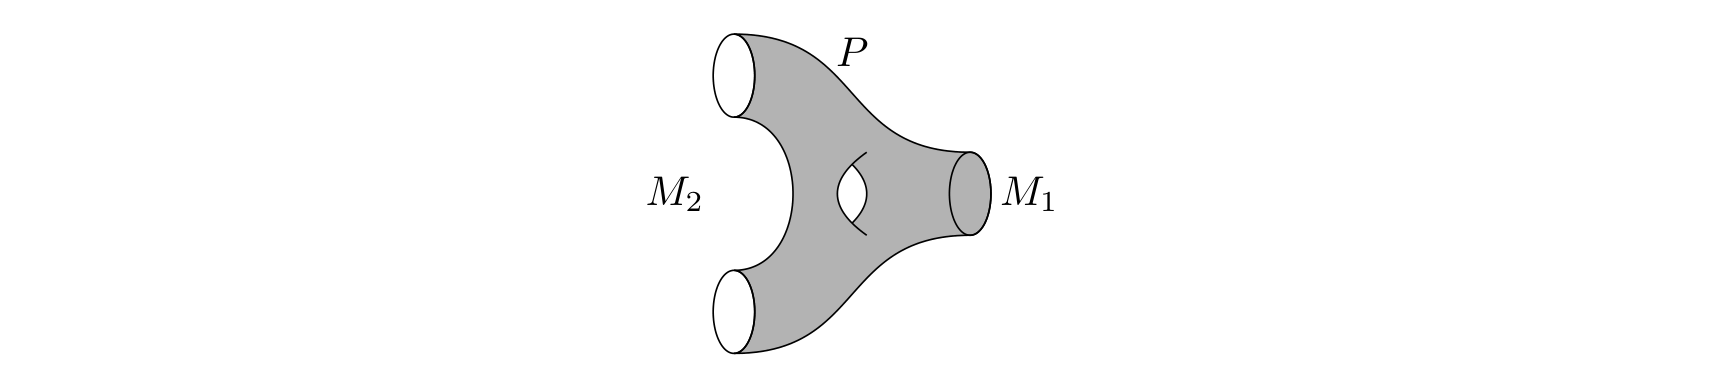
\includegraphics[width=0.58\textwidth]{figure6-1.png}
  \caption{两个对象（闭 $(n-1)$-流形）$M_1$ 与 $M_2$ 之间在 $\Bord_{n-1,n}$ 中的一个态射，
  是以为 $M_1\sqcup M_2$ 边界的 $n$-流形 $P$。（原文 p.~78，Figure 6.1）}
  \label{fig:6-1}
\end{figure}

\begin{figure}[htbp]
  \centering
  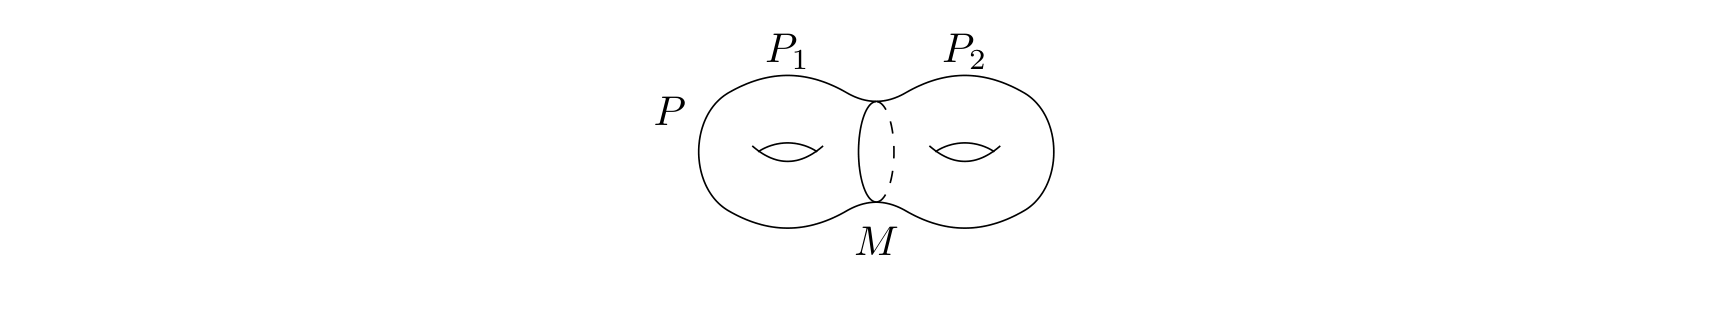
\includegraphics[width=0.55\textwidth]{figure6-2.png}
  \caption{闭 $n$-流形分解为沿 $M$ 相交的两块 $P_1$ 与 $P_2$。（原文 p.~78，Figure 6.2）}
  \label{fig:6-2}
\end{figure}

\subsection{Atiyah--Segal TFT}

一个 Atiyah--Segal（非扩展）TFT 是对称幺半函子
\begin{equation}\tag{6.22}\label{eq:6.22}
\bigl(\Bord_{n-1,n},\sqcup\bigr)\xrightarrow{\ Z\ }\bigl(\Vect,\otimes\bigr).
\end{equation}
$\Bord_{n-1,n}$ 的对象是（定向的\footnote{我们可以要求配边带有不同的切结构；这里只取定向的。}）
闭 $(n-1)$-流形。$\Vect$ 的对象是（复）向量空间。于是闭 $(n-1)$-流形 $M$ 送到某个向量空间 $Z(M)$。
$\Bord_{n-1,n}$ 中的态射 $P\colon M_1\to M_2$ 是一个 $n$-流形 $P$，其边界
$\partial M=M_1\sqcup M_2$，如图 \ref{fig:6-1}。

要理解为什么应该这样想，我们需要把注意力从状态向量空间移开，暂时重新聚焦于闭 $n$-流形 $P$ 上的
配分函数 $Z(P)$。想法是：Atiyah--Segal 对 TFT 的这种形式化，编码了配分函数的局部性。
也就是说，若把 $P$ 切成两块 $P_1$ 与 $P_2$ 并沿 $M$ 粘合（如图 \ref{fig:6-2}），
则 $Z(P)$ 分解为
\diageq{6.23}{0.42\textwidth}{p078_d3.png}

我们更关心 $(n-1)$-流形 $M$ 上的状态向量空间。想法是同样可以把 $Z(M)$ 分解为来自 $M$ 的分解的
“局部块”：
\begin{equation}\tag{6.24}\label{eq:6.24}
M=M_1\sqcup_N M_2,
\end{equation}
其中 $N$ 的余维为 2。我们希望写成
\begin{equation}\tag{6.25}\label{eq:6.25}
Z(M)=\bigl\langle Z(M_1),Z(M_2)\bigr\rangle_{Z(N)},
\end{equation}
但 Atiyah--Segal 形式化没有告诉我们如何做到这一点。这正是扩展场论的基本想法，
它归功于 Freed、Lawrence、Baez--Dolan 等（原文此处只标注了 “cite”，未给出具体文献）。

% [Tutor Note: 式 (6.25) 中的 $\langle-,-\rangle_{Z(N)}$ 是范畴中的 Hom/张量配对（在 2-范畴里即
%  “沿 $Z(N)$ 的态射空间”），不是 Hilbert 空间的内积。若把 $Z(N)$ 想成 $\Shv(\cF(N))$，
%  则这个配对就是层范畴中的 $\otimes_{\Shv(\cF(N))}$ 与 Hom。作者用尖括号是为了提示与
%  向量空间内积的类比，但切勿按内积（共轭线性）理解。]

\begin{figure}[htbp]
  \centering
  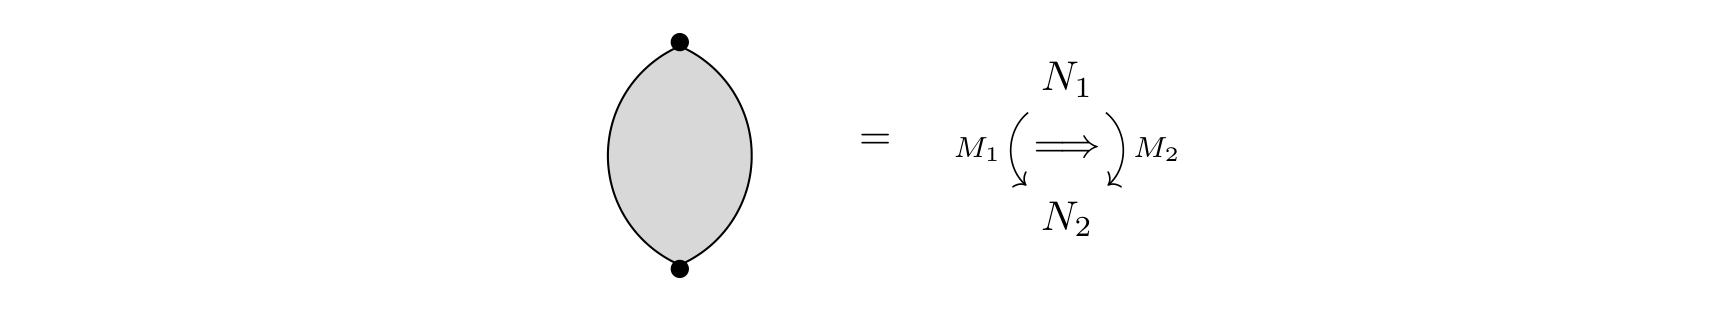
\includegraphics[width=0.6\textwidth]{figure6-3.png}
  \caption{这个带角的流形是 $\Bord_{0,2}$ 中两个 1-态射之间的一个 2-态射。（原文 p.~79，Figure 6.3）}
  \label{fig:6-3}
\end{figure}

基本上，我们需要把某种对象附着到余维 2 的空间。

为形式化这一点，我们定义某种 2-范畴 $\Bord_{n-2,n}$。对象是闭 $(n-2)$-流形 $N$，
态射是以 $N_1\sqcup N_2$ 为边界的 $(n-1)$-流形，2-态射是带角的 $n$-流形。
两个 1-态射之间 2-态射的例子见 $\Bord_{0,2}$ 中的图 \ref{fig:6-3}。

2-层 TFT 是对称幺半函子
\begin{equation}\tag{6.26}\label{eq:6.26}
Z\colon\bigl(\Bord_{n-2,n},\sqcup\bigr)\to\bigl(\cC,\otimes\bigr),
\end{equation}
其中 $(\cC,\otimes)$ 是某个对称幺半 2-范畴。除对称幺半外，我们还希望这个函子如下地还原
“1-层”（即 Atiyah--Segal）形式化。空 $(n-2)$-流形 $\emptyset_{n-2}$ 是 $\Bord_{n-2,n}$ 的单位。
函子是对称幺半的，意味着它被送到单位 $1\in\cC$。空 $(n-2)$-流形的自同态是
\begin{equation}\tag{6.27}\label{eq:6.27}
\End_{\Bord_{n-2,n}}\bigl(\emptyset_{n-2}\bigr)=\Bord_{n,n-1},
\end{equation}
因为空 $\{n-2\}$-流形到自身的配边由闭 $(n-1)$-流形组成。于是我们可能要求 $\cC$ 是 $\Vect$ 的
一个\term{去环路}{delooping}。这只是说
\begin{equation}\tag{6.28}\label{eq:6.28}
\End_{\cC}(1_{\cC})=\Vect .
\end{equation}
此时函子 $Z$ 决定了映射
\begin{equation}\tag{6.29}\label{eq:6.29}
\End_{\Bord_{n-2,n}}\bigl(\emptyset_{n-2}\bigr)=\Bord_{n,n-1}\to\Vect=\End(1_{\cC}).
\end{equation}

无论 $\cC$ 是什么，我们都得到想要的局部性：若 $M=M_1\sqcup_N M_2$，则函子性告诉我们
\begin{equation}\tag{6.30}\label{eq:6.30}
\begin{array}{ccc}
1_{\cC} & \xrightarrow{\ Z(M_1)\ } Z(N) \xrightarrow{\ Z(M_2)\ } & 1_{\cC}\\[6pt]
& \Downarrow{\scriptstyle Z(M)} &
\end{array}
\end{equation}

$\cC$ 的一个自然选择是 $\mathrm{Cat}_{\C}$。其对象是 $\Vect_{\C}$ 上的充实范畴，
1-态射是线性函子，2-态射是线性自然变换。还有别的选择，但这在某种意义下是最基本的一个。
现在我们要把场论延拓到余维 2，以编码分歧。也就是说，我们想要一种方式把余维 2 的 $N$
附着到某个范畴，并（非正式地）把它想成 $\Shv(\cF(N))$。

设 $M$ 是闭 3-流形，$Z$ 是 4 维 TFT，$K\subset M$ 是一个纽结。那么管状纽结的补集 $M_0$ 有边界
$\partial M_0=N$。于是这给出函子
\begin{equation}\tag{6.31}\label{eq:6.31}
Z(N)\xrightarrow{\ Z(M_0)\ } Z(\emptyset)=\Vect .
\end{equation}

% [Tutor Note: 式 (6.27)--(6.29) 是“去环路”条件的标准表述，但 2-范畴 $\cC$ 的环路
%  $\End_\cC(1_\cC)$ 只在 $\cC$ 是单对象 2-范畴（即带 $E_1$ 结构的幺半范畴）时才是通常意义的
%  幺半范畴。此处作者取 $n=2$ 的例子（$\Bord_{0,2}$）作直观；对一般的 $n$，$\Bord_{n-2,n}$
%  是 $n$-范畴，去环路需迭代。严格的完全扩展 TFT 由配边假设（cobordism hypothesis，
%  Lurie）刻画：$Z$ 由 $Z(\mathrm{pt})$ 作为可对偶对象唯一决定。建议对照 [Lur09] 第 2.3 节。]

想法是：我们从某个向量空间 $Z(M)$ 出发，沿边界按某个条件修改它，得到向量空间 $Z(M_0)$。

我们去掉的东西的内部，即纽结的环面邻域，记作 $M_1$，它定义了函子 $\Vect\to Z(N)$；
函子性给出
\begin{equation}\tag{6.32}\label{eq:6.32}
\begin{array}{ccc}
\Vect & \xrightarrow{\ Z(M_1)\ } Z(N) \xrightarrow{\ Z(M_0)\ } & \Vect\\[6pt]
& \Downarrow{\scriptstyle Z(M)} &
\end{array}
\end{equation}
这就是扩展场论编码我们一直讨论的边界条件的方式。

\section{阿贝尔对偶的例子}

\begin{sectionkey}
本节把第 3 章的两个二维阿贝尔对偶例子放到余维 2 的分歧下重新审视：A-侧的场空间由同伦型决定，
B-侧必须取栈（而不能只取同构类），于是“点”上的范畴一边是分次向量空间、另一边是 $\C^\times$ 的表示；
这两者由 Fourier 对偶（Pontrjagin 对偶的范畴化）等同。
\end{sectionkey}

回忆第 3 章的阿贝尔对偶。特别是第 3.7.2 节、第 3.7.3 节与第 4.6 节中的二维例子。
现在我们在这些例子中加入余维 2 的分歧来讨论。

\subsection{二维情形}

回忆第一个例子把 A-侧的 $H^0(S^1,\Z)$ 与 B-侧的 $H^1(S^1,\C^{\times})$ 交换。
在 A-侧，场由
\begin{equation}\tag{6.33}\label{eq:6.33}
\cF(-)=\operatorname{Maps}(-,\Z)
\end{equation}
给出，故在连通流形上场看起来就是 $\Z$。唯一余维为 2 的子流形是点，而附着到点的范畴是
\begin{equation}\tag{6.34}\label{eq:6.34}
Z(\mathrm{pt})=\Shv(\Z)=\Vect^{\Z\text{-gr}},
\end{equation}
即分次向量空间的范畴。

在 B-侧，我们把 $H^1(S^1,\C^{\times})$ 解释为 $S^1$ 上 $\C^{\times}$-局部系统的同构类。
这建议我们的场空间应该是
\begin{equation}\tag{6.35}\label{eq:6.35}
\cF(-)=\Loc_{\C^{\times}}(-).
\end{equation}
若真的只考虑同构类构成的集合，我们不会得到附着到点的范畴：$\Loc_{\C^{\times}}(\mathrm{pt})$
只是单点，故与另一侧不匹配。相反，我们必须把它想成一个栈。它仍然是点，
但带 $\C^{\times}$ 通过自同构的作用。也就是说，它是栈
\begin{equation}\tag{6.36}\label{eq:6.36}
B\C^{\times}=\mathrm{pt}/\C^{\times}.
\end{equation}
取层时得到
\begin{equation}\tag{6.37}\label{eq:6.37}
\Shv\bigl(\cF(\mathrm{pt})\bigr)=\Shv\bigl(\mathrm{pt}/\C^{\times}\bigr)
=\Rep\bigl(\C^{\times}\bigr)\simeq\Vect^{\Z\text{-gr}}.
\end{equation}
$\C^{\times}$ 的表示与分次向量空间之间的等同如下给出。给定 $\C^{\times}$ 的表示 $V$，得到分次
\begin{equation}\tag{6.38}\label{eq:6.38}
V=\bigoplus_{n\in\Z}V_n,
\end{equation}
其中 $V_n$ 是 $z\in\C^{\times}$ 以 $z^n$ 作用的部分。

% [Tutor Note: (6.36)--(6.37) 是本章的关键机制，也是初学者最容易出错的地方：
%  $\Loc_{\C^\times}(\mathrm{pt})$ 作为集合只是一个点，但作为栈它是 $B\C^\times=\mathrm{pt}/\C^\times$，
%  其上的拟凝聚层/局部系统给出 $\Rep(\C^\times)\simeq\Vect^{\Z\text{-gr}}$。
%  若在 A-侧同样只取同构类，就丢掉了 $\Z$-分次结构，两边不可能等同。
%  另外需注意：$\Shv(\Z)$ 这里指 $\Z$（离散群）上局部系统的范畴，等价于分次向量空间，
%  而不是 $\Z$ 上层的导出范畴。]

我们可以如下把它看成 Pontrjagin 对偶的某种版本。可以把 $\Shv(\Z)$ 想成带逐点乘法的
$\C[\Z]$ 的模：
\begin{equation}\tag{6.39}\label{eq:6.39}
\Shv(\Z)=(\C[\Z],\cdot)\text{-mod}.
\end{equation}
对偶地，$\C^{\times}$ 的表示可以想成带卷积的 $\C[\C^{\times}]$ 的模：
\begin{equation}\tag{6.40}\label{eq:6.40}
\Rep\bigl(\C^{\times}\bigr)=(\C\C^{\times},*)\text{-mod}.
\end{equation}
这一对偶断言这两个范畴等价。在 B-侧我们真正看的是 $\C^{\times}$ 上代数函数的余模，
即 $\C[\C^{\times}]$-comod；也就是说，$\Z$ 上函数的模是 $\C^{\times}$ 上函数的余模。

\subsection{二维情形}

回忆第 3.7.3 节与第 4.6 节，那里讨论了二维阿贝尔对偶的另一个例子。A-侧由 $H^1(S^1,\Z)$ 上的
函数给出，B-侧由 $H^0(S^1,\C^{\times})$ 上的函数给出。这是 T-对偶或镜像对称的基本例子。

在 A-侧，我们可以把它想成
\begin{equation}\tag{6.41}\label{eq:6.41}
H^1(S^1,\Z)=H^0(S^1,B\Z).
\end{equation}
这建议场空间由
\begin{equation}\tag{6.42}\label{eq:6.42}
\cF(-)=\operatorname{Maps}\bigl(-,B\Z=S^1\bigr)
\end{equation}
给出，故
\begin{equation}\tag{6.43}\label{eq:6.43}
\cF(\mathrm{pt})=S^1=B\Z .
\end{equation}
于是所要的范畴是它上面的某种层，我们取为局部常值的：
\begin{equation}\tag{6.44}\label{eq:6.44}
\Shv(B\Z):=\Loc(S^1)=\Rep(\Z)=(\C\Z,*)\text{-mod}.
\end{equation}
这个范畴的另一个名字是 $T^*S^1$ 的（卷绕）Fukaya 范畴。要点是：$T^*S^1$ 的辛拓扑就是
$S^1$ 的普通拓扑。

在 B-侧，圆周上的场由 $H^0(S^1,\C^{\times})$ 给出，这告诉我们场是到带离散拓扑的 $\C^{\times}$ 的映射：
\begin{equation}\tag{6.45}\label{eq:6.45}
\cF(-)=\operatorname{Maps}\bigl(-,\C^{\times}_{\mathrm{disc}}\bigr).
\end{equation}
特别地，
\begin{equation}\tag{6.46}\label{eq:6.46}
\cF(\mathrm{pt})=\C^{\times},
\end{equation}
而自然的层范畴将是拟凝聚的\footnote{这与 A-侧我们所用的局部常值层形成对比。}：
\begin{equation}\tag{6.47}\label{eq:6.47}
\Shv_B\bigl(\C^{\times}\bigr):=\QC\bigl(\C^{\times}\bigr)
=(\C[\C^{\times}],\cdot)\text{-mod}
=\C[z,z^{-1}]\text{-mod}.
\end{equation}

% [Tutor Note: 原文第 6.3 节的两个子节标题都写作 “Two-dimensions”，这是作者的重复，
%  并非排版偶然（源文 p.79 与 p.80 均如此）。这里按原文照译，便于对照；
%  内容上两小节分别处理 $H^0\leftrightarrow H^1$ 与 $H^1\leftrightarrow H^0$ 两组对偶。]

再次看到，这在模仿我们在 Pontrjagin 对偶情形所见。在 A-侧我们有带卷积的 $\C[\Z]$ 的模，
在 B-侧我们有带逐点乘法的 $\C[\C^{\times}]$ 的模。

换言之，可以把 $\C[z,z^{-1}]$ 想成 $\C^{\times}$ 上的函数，或想成 $\Z$ 的群代数 $\C[\Z]$：
\begin{equation}\tag{6.48}\label{eq:6.48}
\text{$\C^{\times}$ 上的函数}=\C[z,z^{-1}]=\C[\Z],
\end{equation}
故一个模既可以看作圆周上的局部系统，也可以看作 $\C^{\times}$ 上的层。

这是同调镜像对称的第一个例子：
\begin{equation}\tag{6.49}\label{eq:6.49}
\operatorname{Fuk}^{wr}\bigl(T^*S^1\bigr)=\Loc(S^1)\simeq\QC\bigl(\C^{\times}\bigr).
\end{equation}

\section{四维 Maxwell 理论}

\begin{sectionkey}
本节把四维拓扑 Maxwell 理论的对偶降到余维 2（曲面）：A-侧的 $\operatorname{Pic}\Sigma$
与 B-侧的 $\C^\times$-局部系统 $\Loc_{\C^\times}(\Sigma)$ 上的层范畴，经由 Fourier--Mukai 变换等同；
这也给出 $G=\mathrm{GL}_1$ 的 Betti 几何 Langlands 对应的一个初等例子。
\end{sectionkey}

回忆第 4.8.1 节的四维 Maxwell 理论。这个对偶把 A-侧线丛的拓扑与 B-侧平坦线丛的代数几何交换。
回忆这个对偶把 A-侧的 $H^2(M^3,\Z)$ 与 B-侧的 $H^1(M^3,\C^{\times})$ 交换。
现在我们要把第 4.5.1 节中余维 1 的缺陷降到余维 2，即降到曲面。

\subsection{A-侧}

设 $\Sigma$ 是曲面。在 A-侧我们有
\begin{equation}\tag{6.50}\label{eq:6.50}
H^2(-,\Z)=\pi_0\Bigl(\operatorname{Map}\bigl(-,\underbrace{BU(1)}_{K(\Z,2)}\bigr)\Bigr),
\end{equation}
即我们在探测某个更大对象的连通分量。这建议我们的场应该类似
\begin{equation}\tag{6.51}\label{eq:6.51}
\cF(-)=\operatorname{Map}\bigl(-,BU(1)\bigr).
\end{equation}
我们把这些记作 $\operatorname{Pic}\Sigma$：
\begin{equation}\tag{6.52}\label{eq:6.52}
\cF(\Sigma)=\operatorname{Pic}\Sigma:=\operatorname{Map}\bigl(\Sigma,BU(1)\bigr).
\end{equation}
为更清楚地看出与线丛的等同，在 $\Sigma$ 上取一个复结构（于是它现在是 Riemann 面）。
然后可以看 $\Sigma$ 上全纯/代数线丛构成的空间 $\operatorname{Pic}\Sigma$。这是代数几何的对象，
但我们只关心其拓扑。故此空间不依赖复结构，但选一个复结构让我们能显式地实现这个空间。
它适合短正合列
\begin{equation}\tag{6.53}\label{eq:6.53}
0\to\operatorname{Jac}\Sigma\to\operatorname{Pic}\Sigma\xrightarrow{\ \deg\ }\Z\to 0,
\end{equation}
其中 $\operatorname{Jac}\Sigma$ 由 0 次线丛组成。断言是 $\operatorname{Jac}\Sigma$ 是实维 $2g$ 的环面，
故拓扑上它就是
\begin{equation}\tag{6.54}\label{eq:6.54}
\operatorname{Jac}\Sigma\simeq \C^g/\Z^{2g}.
\end{equation}

\begin{srcrem}{27}
我们又一次忽略了这些线丛的自同构，它们会贡献额外的（栈性）因子 $BU(1)$。
\end{srcrem}

我们如下得到显式描述。指数短正合列
\begin{equation}\tag{6.55}\label{eq:6.55}
0\to\Z\to\cO\to\cO^{\times}\to 0
\end{equation}
给出
\begin{equation}\tag{6.56}\label{eq:6.56}
0\to H^1(\Sigma,\cO)/H^1(\Sigma,\Z)\to H^1(\Sigma,\cO^{\times})
\to H^2(\Sigma,\Z)=\Z\to 0,
\end{equation}
故
\begin{equation}\tag{6.57}\label{eq:6.57}
\operatorname{Jac}\simeq K\bigl(H^1(\Sigma,\Z),1\bigr),
\end{equation}
即以 $H^1(\Sigma,\Z)$ 为 $\pi_1$ 的环面。

因此，这个阿贝尔范畴可以写成
\begin{align}
\Loc(\operatorname{Pic}\Sigma)
&=\Vect^{\Z\text{-gr}}\otimes\Loc(\operatorname{Jac}\Sigma)\tag{6.58}\label{eq:6.58}\\
&=\Rep_{\Z\text{-gr}}\bigl(\Lambda=H^1(\Sigma,\Z)\bigr)\tag{6.59}\label{eq:6.59}\\
&=\Vect^{\Z\text{-gr}}\otimes\bigl(\C[H^1(\Sigma,\Z)],*\bigr).\tag{6.60}\label{eq:6.60}
\end{align}

\begin{flushright}
\small 第 12 讲；2021 年 3 月 4 日
\end{flushright}

\subsection{B-侧}

现在我们来检查在 B-侧该做什么，那里我们研究 $\C^{\times}$-局部系统的代数几何。
也就是说，对曲面 $\Sigma$（不必带复结构），我们考虑
\begin{align}
\Loc_{\C^{\times}}(\Sigma)
&=\Hom\bigl(\pi_1(\Sigma),\C^{\times}\bigr)/\C^{\times}\tag{6.61}\label{eq:6.61}\\
&=\Hom\bigl(H_1(\Sigma,\Z),\C^{\times}\bigr)/\C^{\times}\tag{6.62}\label{eq:6.62}\\
&\simeq\bigl(H^1(\Sigma,\Z)\otimes_{\Z}\C^{\times}\bigr)/\C^{\times}.\tag{6.63}\label{eq:6.63}
\end{align}
现在应该附着某种（层）范畴。我们在做代数几何，故自然的层范畴是
\begin{equation}\tag{6.64}\label{eq:6.64}
\QC\bigl(\Loc_{\C^{\times}}\Sigma\bigr)
=\bigl(\C[\Loc_{\C^{\times}}(\Sigma)],\cdot\bigr)\text{-mod}
\otimes\Rep\bigl(\C^{\times}\bigr).
\end{equation}
这个函数环可以写成
\begin{equation}\tag{6.65}\label{eq:6.65}
\C\bigl[\Loc_{\C^{\times}}(\Sigma)\bigr]=\C\bigl[H^1(\Sigma,\Z)\bigr].
\end{equation}
现在由 Poincaré 对偶有 $H^1(\Sigma,\Z)\simeq H_1(\Sigma,\Z)$。又已见
$\Rep\C^{\times}=\Vect^{\Z\text{-gr}}$。

现在可以把这与 A-侧式 \eqref{eq:6.60} 比较。带卷积的格代数 $(\C\Lambda,*)$ 通过 Fourier 级数
与 $(\C[T^{\vee}],\cdot)$ 等同。这意味着这两个代数上的模相同，即
\begin{equation}\tag{6.66}\label{eq:6.66}
\Loc K(\Lambda,1)\simeq\QC\bigl(T^{\vee}_{\C}\bigr).
\end{equation}
这里左端是 $\Loc\operatorname{Jac}(\Sigma)$，右端是 $\QC(\Loc)$ 但忽略了 $\C^{\times}$ 的额外作用。

于是结论是
\begin{equation}\tag{6.67}\label{eq:6.67}
\Loc\operatorname{Pic}(\Sigma)\simeq\QC(\Loc).
\end{equation}
这就是我们对余维 2 的拓扑 Maxwell 理论的阿贝尔对偶。

\begin{srcrem}{28}
这是 Fourier--Mukai 变换的第一个例子，即层范畴的 Fourier 变换版本。
\end{srcrem}

\begin{srcrem}{29}
这是 $G=\mathrm{GL}_1$ 的 Betti 几何\footnote{“几何”只是指我们在范畴层面看问题。}
Langlands 对应的陈述。
\end{srcrem}

% [Tutor Note: 式 (6.56) 的长正合列容易看漏一处：$H^1(\Sigma,\cO)/H^1(\Sigma,\Z)$ 中的
%  $H^1(\Sigma,\Z)$ 通过指数正合列嵌入 $H^1(\Sigma,\cO)$，这一步用的是 $H^2(\Sigma,\Z)=\Z$
%  与 $H^2(\Sigma,\cO)=0$（对紧 Riemann 面）。于是 $\operatorname{Jac}\simeq K(H^1(\Sigma,\Z),1)$，
%  其复结构来自 $H^1(\Sigma,\cO)/H^1(\Sigma,\Z)$。另注意 (6.66) 中对偶环面 $T^{\vee}_{\C}$ 的
%  下标是复数域：这里的“Fourier 对偶”是在复环面层面，$\pi_1$ 与 $H^1$ 互换。]

\subsection{带分歧的电磁对偶}

我们想写出带分歧的一般电磁对偶。这将包括 Dirac 单极子（第 4.5.1 节）与螺线管（第 4.8.2 节）。
回忆曲面 $\Sigma$ 作为 3-流形 $M_0=M\setminus K$ 的边界出现，其中 $K\subset M$ 是一个纽结。

在 A-侧，我们有（限制）映射
\begin{equation}\tag{6.68}\label{eq:6.68}
\operatorname{Pic}(M_0)\xrightarrow{\ \pi\ }\operatorname{Pic}(\Sigma),
\end{equation}
这里我们仍只从拓扑上考虑 $\operatorname{Pic}$。设 $\cE\in\Loc(\operatorname{Pic}\Sigma)$。
则得到
\begin{equation}\tag{6.69}\label{eq:6.69}
\pi^*\cE\in\Loc\bigl(\operatorname{Pic}(M_0)\bigr),
\end{equation}
并且可以附着如下向量空间：
\begin{equation}\tag{6.70}\label{eq:6.70}
\Gamma\bigl(\operatorname{Pic}(M_0),\pi^*\cE\bigr).
\end{equation}
这是我们说“用某些分歧数据修改 $Z(M)$”的方式。

在 B-侧，我们也可以限制
\begin{equation}\tag{6.71}\label{eq:6.71}
\Loc_{\C^{\times}}M_0\xrightarrow{\ \pi^{\vee}\ }\Loc_{\C^{\times}}\Sigma,
\end{equation}
然后可以把 $\cE^{\vee}\in\QC(\Loc_{\C^{\times}}\Sigma)$ 拉回，得到
\begin{equation}\tag{6.72}\label{eq:6.72}
\pi^{\vee*}\cE^{\vee}\in\QC\bigl(\Loc_{\C^{\times}}M_0\bigr),
\end{equation}
并且可以附着如下向量空间：
\begin{equation}\tag{6.73}\label{eq:6.73}
\Gamma\bigl(M_0,\pi^{\vee*}\cE^{\vee}\bigr).
\end{equation}
于是带分歧的电磁对偶通过 Fourier--Mukai 变换交换 $\cE$ 与 $\cE^{\vee}$。特别地，它告诉我们
\begin{equation}\tag{6.74}\label{eq:6.74}
\Gamma\bigl(\operatorname{Pic}M_0^3,\pi^*\cE\bigr)
\simeq\Gamma\bigl(\Loc_{\C^{\times}}M,\pi^{\vee*}\cE^{\vee}\bigr).
\end{equation}
层 $\cE$ 与 $\cE^{\vee}$ 规定边界条件，例如 Dirichlet 或 Neumann。例如 $\cE^{\vee}$ 可能是
$\Loc_{\C^{\times}}(\Sigma)$ 中某个轨迹的结构层。于是我们看的是沿该轨迹带有特定奇点的局部系统，
即 $\Loc M_0$ 中那些限制到边界 $\Sigma$ 后落到特定子集的元素。

% [Tutor Note: 式 (6.74) 的记号与上下文不完全一致：左端的 $M_0^3$ 应即三维流形 $M_0$（上标 $3$
%  表示维数），右端的 $\Loc_{\C^{\times}}M$ 按限制映射 (6.71) 的源应为 $\Loc_{\C^{\times}}M_0$
%  （去掉纽结后的流形），而不是整个 $M$。作者混用了 $M$ 与 $M_0$。理解时以 (6.73) 为准：
%  两边分别是 $\Gamma(\operatorname{Pic}(M_0),\pi^*\cE)$ 与 $\Gamma(M_0,\pi^{\vee*}\cE^{\vee})$。]

\section{带分歧的类域论}

\begin{sectionkey}
本节把 3-流形/纽结的拓扑图景平移到曲线 $C/\F_q$ 与其上一点 $x$：$K_x^\times$ 的作用代替了
边界层的拉回，局部类域论给出 $K_x^\times$ 的表示与 $D_x^\times$ 上秩 1 局部系统（即
$\Gal(\overline{K}_x/K_x)$ 的特征）的对偶，而整体类域论把 $\operatorname{Pic}$ 的“带水平结构版本”
与在 $S$ 处分歧的 Galois 特征对应起来。
\end{sectionkey}

设 $C/\F_q$ 是有限域上的曲线。对点 $x\in C$，我们想在这一点“允许分歧”。
考虑分歧曲线内 $x$ 周围的穿孔圆盘：
\begin{equation}\tag{6.75}\label{eq:6.75}
\Spec K_x=D_x^{\times}\hookrightarrow C\setminus x .
\end{equation}
注意 $K_x\simeq \F_q((t))$。这幅图是“管状邻域的边界位于 3-流形内部”的类比：
\begin{equation}\tag{6.76}\label{eq:6.76}
N=\partial\bigl(\text{$K$ 的管状邻域}\bigr)\hookrightarrow M_0=M\setminus K .
\end{equation}
所以现在切除的是点（而不是纽结），并且我们要理解的是这个穿孔圆盘，
而不是纽结管状邻域的边界。

在 B/Galois 侧，我们看的是 $\Loc_1(C\setminus x)$。无论这些是什么，它们都可以限制到穿孔圆盘：
\begin{align}
\Loc_1(C\setminus x)\to\Loc_1 D^{\times}
&=\Hom_{cts}\bigl(\Gal(\overline{K}_x/K_x),\overline{\Q}_{\ell}^{\times}\bigr)\tag{6.77}\label{eq:6.77}\\
&=\Hom_{cts}\bigl(\Gal^{ab}(\overline{K}_x/K_x),\overline{\Q}_{\ell}^{\times}\bigr).\tag{6.78}\label{eq:6.78}
\end{align}
也就是说，我们研究的是 Abel 化 Galois 群的特征，但它们作为 $D^{\times}$ 上的局部系统出现。
于是现在的想法是：研究 $C\setminus x$ 上带有绕该穿孔点的特定分歧数据的局部系统。

在 A-侧，我们看的是 $\operatorname{Pic}C$。回忆第 5.2.2 节中它的阿黛尔描述：
\begin{align}
\operatorname{Pic}C
&=F^{\times}\Big\backslash\sideset{}{'}\prod_{y\in C}K_y^{\times}
\Big/\prod_{y\in C}\cO_y^{\times}\tag{6.79}\label{eq:6.79}\\
&=F^{\times}\Big\backslash\sideset{}{'}\prod\Z .\tag{6.80}\label{eq:6.80}
\end{align}
对穿孔曲线有类似的描述：
\begin{equation}\tag{6.81}\label{eq:6.81}
\operatorname{Pic}(C\setminus x)
=F^{\times}\Big\backslash\sideset{}{'}\prod_{y\in C\setminus x}K_y^{\times}
\Big/\prod_{y\in C\setminus x}\cO_y^{\times}.
\end{equation}
我们可以把它写成
\begin{align}
\operatorname{Pic}(C\setminus x)
&=F^{\times}\Big\backslash\sideset{}{'}\prod_{y\in C\setminus x}K_y^{\times}
\Big/\prod_{y\in C\setminus x}\cO_y^{\times}\tag{6.82}\label{eq:6.82}\\
&=\operatorname{Pic}C\Big/\bigl(\Z_x=K_x^{\times}/\cO_x^{\times}\bigr),\tag{6.83}\label{eq:6.83}
\end{align}
这里我们模掉的是“加减这个点 $x$ 的拷贝”。然后也可以把它写成
\begin{align}
\operatorname{Pic}(C\setminus x)
&=F^{\times}\Big\backslash\sideset{}{'}\prod_{y\in C\setminus x}K_y^{\times}
\Big/\prod_{y\in C\setminus x}\cO_y^{\times}\tag{6.84}\label{eq:6.84}\\
&=\operatorname{Pic}C\Big/\bigl(\Z_x=K_x^{\times}/\cO_x^{\times}\bigr)\tag{6.85}\label{eq:6.85}\\
&=\operatorname{Pic}(C,\widehat{x})\big/K_x^{\times},\tag{6.86}\label{eq:6.86}
\end{align}
其中 $\operatorname{Pic}(C,\widehat{x})$ 定义为 $C$ 上配备 $D_x$ 上平凡化的线丛。
故我们在右边模掉这个平凡化。

$\operatorname{Pic}(C,\widehat{x})$ 映到 $\operatorname{Pic}C$，其纤维由平凡化的改变给出，
并有中间对象 $\operatorname{Pic}(C,nx)$（$n\in\Z^{+}$）：
\begin{equation}\tag{6.87}\label{eq:6.87}
\begin{array}{ccc}
\operatorname{Pic}(C,\widehat{x}) & \xrightarrow{\ \cO_x^{\times}\ } & \operatorname{Pic}(C)\\[2pt]
\searrow & & \nearrow\\[2pt]
& \operatorname{Pic}(C,nx) &
\end{array}
\end{equation}
其中 $\operatorname{Pic}(C,nx)$ 由 $\operatorname{Pic}(C)$ 中在 $x$ 周围有 $n$ 阶平凡化的对象组成。
这个说法告诉我们：要研究穿孔曲线，并不需要真的穿孔。只要理解 $K_x^{\times}$ 如何作用，
就可以研究 $C$ 上配备平凡化的丛。

% [Tutor Note: 原文 (6.81)--(6.86) 有重复排版：式 (6.81) 与 (6.82) 的左端表达式相同，
%  (6.84) 与 (6.82)、(6.85) 与 (6.83) 分别重复（源文 p.84--85）。这里照原文保留，
%  只为便于对照；逻辑上只需 (6.81)--(6.83) 与 (6.86)。另外 (6.79) 中的 $\prod'$ 表示
%  限制直积：除有限多个因子外，$K_y^{\times}$ 的因子都落在 $\cO_y^{\times}$ 中。]

无论如何，$\operatorname{Pic}(C,\widehat{x})$ 上有 $K_x^{\times}$ 的作用。所以我们将看
$\operatorname{Pic}(C,\widehat{x})$ 上的函数，并在这个作用下分解它们。从 TFT 的观点，
我们说得略有不同。也就是说，我们有限制
\begin{equation}\tag{6.88}\label{eq:6.88}
\begin{array}{ccc}
\operatorname{Pic}(C\setminus x) & = & \operatorname{Pic}(C,\widehat{x})/K^{\times}\\[2pt]
\downarrow & & \downarrow\\[2pt]
\operatorname{Pic}(D_x^{\times}) & = & \mathrm{pt}/K^{\times},
\end{array}
\end{equation}
并且可以取一个层并在 $\operatorname{Pic}(C,\widehat{x})$ 上取整体截面，即前推到 $\mathrm{pt}/K_x^{\times}$。
研究这幅图等价于研究 $K^{\times}$ 在 $\operatorname{Pic}(C,\widehat{x})$ 上的作用。

数论学家会告诉你，你不想要“无限水平结构”。我们有 $K=\F_q((t))$。于是
\begin{equation}\tag{6.89}\label{eq:6.89}
K^{\times}=\F_q((t))^{\times}\supset\cO^{\times}=\F_q[[t]].
\end{equation}
它还包含这些子群：
\begin{equation}\tag{6.90}\label{eq:6.90}
K^{\times}\supset\cO^{\times}\supset\cO^{\times(1)}\supset\cdots\supset\cO^{\times(n)}\supset\cdots
\end{equation}
其中属于 $\cO^{\times(n)}$ 只意味着你形如 $(1+t^n)(-)$。

之前，商 $K^{\times}/\cO^{\times}=\Z$ 给我们除子。故在非分歧情形，我们有 $\Z$ 作用在
$\operatorname{Pic}(C)$ 上。现在当我们添加水平结构，即从 $\operatorname{Pic}(C)$ 过渡到
$\operatorname{Pic}(C,nx)$ 时，我们有 $K^{\times}/\cO^{\times(n)}$ 的作用。

所以我们做的是看 $K^{\times}$ 的\term{光滑表示}{smooth representation}，即每个向量都被某个
$\cO^{\times(N)}$（$N\gg 0$）固定。若给它作用的那个东西以离散拓扑，这等价于拓扑连续性。

现在要建立如下图景的类比：对以 $\partial M_0=\Sigma$ 为边界的 3-流形 $M_0$，我们得到
\begin{equation}\tag{6.91}\label{eq:6.91}
Z(M_0)\in Z(\Sigma).
\end{equation}
这里的类比如下。对 $C/\F_q$ 与 $x\in C$，我们可以附着
\begin{equation}\tag{6.92}\label{eq:6.92}
\operatorname{Pic}(C,\widehat{x}).
\end{equation}
现在我们要考虑
\begin{equation}\tag{6.93}\label{eq:6.93}
\C\bigl[\operatorname{Pic}(C,\widehat{x})\bigr],
\end{equation}
具体地把它想成 $K_x^{\times}$ 的表示。这可以看作取常值层 $k_{\operatorname{Pic}(C\setminus x)}$
并前推，得到
\begin{equation}\tag{6.94}\label{eq:6.94}
\pi_*k\in\Shv\bigl(\mathrm{pt}/K^{\times}\bigr)=\operatorname{Pic}\bigl(D^{\times}\bigr),
\end{equation}
即 $K^{\times}$ 的一个表示。

于是在 A-侧，我们有来自带无限水平结构的 $\operatorname{Pic}$（即 $\operatorname{Pic}(C,\widehat{x})$，
或某个有限水平结构 $\operatorname{Pic}(C,nx)$）的 $K^{\times}$ 表示。

在 B-侧，我们有层 $\cO_{\Loc(C\setminus x)}$，把它前推得到 $\Loc_1(D^{\times})$ 上的层，
即 $D^{\times}$ 上函数的模。现在我们需要注 28 中 Fourier--Mukai 变换的类比。

这正是局部类域论的内容。

整体类域论说
\begin{equation}\tag{6.95}\label{eq:6.95}
\Gal^{ab,ur}\simeq\widehat{\operatorname{Pic}},
\end{equation}
其中 $\widehat{\operatorname{Pic}}$ 表示 profinite 完备化。局部类域论的陈述是：存在典范映射
\begin{equation}\tag{6.96}\label{eq:6.96}
K_x^{\times}\to\Gal^{ab}\bigl(\overline{K}_x/K_x\bigr),
\end{equation}
它在 profinite 完备化之后是同构：
\begin{equation}\tag{6.97}\label{eq:6.97}
\widehat{K_x^{\times}}\xrightarrow{\ \sim\ }\Gal^{ab}\bigl(\overline{K}_x/K_x\bigr).
\end{equation}
这告诉我们，$K^{\times}$ 的群环与如下对象 Pontrjagin 对偶：
\begin{equation}\tag{6.98}\label{eq:6.98}
\Hom\bigl(\Gal^{ab}(\overline{K}_x/K_x),\overline{\Q}_{\ell}^{\times}\bigr)
=\Hom\bigl(\Gal(\overline{K}_x/K_x),\overline{\Q}_{\ell}^{\times}\bigr)
=\Loc_1(C).
\end{equation}
换言之，
\begin{equation}\tag{6.99}\label{eq:6.99}
\bigl(\overline{\Q}_{\ell}^{\times}[K^{\times}],*\bigr)
\simeq\bigl(\overline{\Q}_{\ell}^{\times}[\Loc_1],\cdot\bigr).
\end{equation}
这类似于在 Riemann 面情形我们把 $\pi_1\operatorname{Jac}=\Lambda$ 与 $\C[T^{\vee}]$ 交换。
现在过渡到模，得到
\begin{equation}\tag{6.100}\label{eq:6.100}
\Rep\bigl(K^{\times}\bigr)=\QC(\Loc_1 C).
\end{equation}
要把这样的陈述在技术上精确化需要大量工作。故局部陈述是：穿孔圆盘上的局部系统与
$K^{\times}$ 的表示有关。而整体陈述是：附着到穿孔曲面的向量空间，即 $K^{\times}$ 的表示，
等同于带有指定分歧的局部系统。

% [Tutor Note: 式 (6.98) 末项在原文中写作 $\Loc_1(C)$（源文 p.86）。按上下文，这里应是
%  $K_x$ 的局部域对应，即 $D_x^{\times}$（或 $C\setminus x$）上秩 1 局部系统的范畴
%  $\Loc_1(D_x^{\times})=\Loc_1(C\setminus x)$，而不是整条曲线 $C$ 上的 $\Loc_1(C)$。
%  这可能是作者把 $C$ 与 $C\setminus x$（或 $D^\times$）混写；同类混写在 (6.74) 中也出现过。
%  另外 (6.95) 的 $\Gal^{ab,ur}$ 是整体类域论中的“非分歧 Abel 化 Galois 群”，
%  而 (6.96)--(6.97) 是局部对应，二者不可混用。]

\section{数域的分歧}

\begin{sectionkey}
本节把上一节的函数域图景逐字搬到数域：局部类域论给出 $K_v^{\times}$ 到局部 Abel 化 Galois 群的
典范映射（在 profinite 完备化后为同构），整体类域论则把带 $S$ 外非分歧条件的阿黛尔商与
在 $S$ 处分歧的 Galois 特征对应起来。
\end{sectionkey}

对数域，陈述非常相似。局部类域论说：对 $F$ 的非 Archimedes 位 $v$，即 $\cO_F$ 中的一个素元，
存在自然映射
\begin{equation}\tag{6.101}\label{eq:6.101}
K_v^{\times}\to\Gal^{ab}\bigl(\overline{K}/K\bigr),
\end{equation}
它在 profinite 完备化上是同构：
\begin{equation}\tag{6.102}\label{eq:6.102}
\widehat{K_v^{\times}}\xrightarrow{\ \sim\ }\Gal^{ab}\bigl(\overline{K}/K\bigr).
\end{equation}
我们可以把这理解为：把 $K^{\times}$ 的表示与 $\mathrm{GL}_1$ 上的函数模、以及 Galois 表示
等同起来（例如取 $K_v=\Q_p$）。

整体类域论说如下。$\operatorname{Pic}(C,\widehat{x})$ 的类比是
\begin{equation}\tag{6.103}\label{eq:6.103}
F^{\times}\Big\backslash\prod_v K^{\times}\Big/\prod_{v\notin S}\cO^{\times},
\end{equation}
而这个东西上的函数带有
\begin{equation}\tag{6.104}\label{eq:6.104}
\prod_{v\in S}K_v^{\times}
\end{equation}
的作用。故我们可以在这个作用下分解它们。这将与在 $S$ 处分歧的 Galois 群的特征（上的函数）相匹配。

% [Tutor Note: 原文 (6.103)--(6.104) 中 $S$ 的含意需要小心：$S$ 是“允许分歧”的有限位集，
%  故在 $S$ 外取整（$\prod_{v\notin S}\cO^{\times}$），而作用来自 $S$ 内的 $K_v^{\times}$。
%  注意 (6.103) 中 $\prod_v$ 的上标 $'$（限制直积）在原文 p.87 被省略，严格写法应为
%  $F^{\times}\backslash\prod'_v K^{\times}/\prod_{v\notin S}\cO^{\times}$。
%  此外 p.87 的原文把 “E.g.\ think $K_v=\Q_p$” 插在句子中间，导致 “representations of
%  $K^\times$ with modules for functions on $\mathrm{GL}_1$ Galois representations” 一句
%  语序破碎；这里按数学含义译出，但源文的断句确实可疑。]

\begin{flushright}
\small 第 13 讲；2021 年 3 月 9 日
\end{flushright}
